To reach the low reaction temperatures desired for our experiment, we need both a cold molecule source as well as a cold and controlled ion source. We may trap \ce{Be+} ions, but given the trap depth of 3 eV, the range of reaction temperatures is vast. Using laser cooling of translational modes of the ions on a closed transition allows us cool down the ion such that clouds and crystals form with temperatures not exceeding 500 mK.\cite{Wineland1979}

Our atom of choice is \ce{^9Be}, which is the only stable isotope of beryllium with a nuclear spin of $I=3/2$. Being an alkaline earth atom, \ce{^9Be} has two valence electrons, and by stripping one off, we are left with an ion with a structure very similar to those of alkali atoms. The states of interest for our work are the \ce{^2S1/2} ground state and \ce{^2P3/2} excited state. In the ground state, the hyperfine splitting between the lower $F=2$ and $F=1$ manifolds is 1.25 GHz \ref{Wineland1983}. Defining the cooling transition on the \ce{^2P3/2} state from the $F=2$ ground manifold allows one to access a stretch transition between the ground $m_F=2$ to excited $m_F'=3$ states with magnetic fields on the order of $2 \times 10^{-5}$ T.\ref{Langer2006} In principle, this scheme does not require any repumping out of the $S$ orbital $F=1$ manifold. Our apparatus does not easily accommodate magnetic field coils necessary to resolve the hyperfine states, requiring repumping out of the $F=1$ manifold. Acousto-optic modulators (AOMs) driven at 400 MHz are used to bridge the 1.25 GHz hyperfine splitting.

Addressing the \ce{^2S1/2 -> ^2P3/2} transition is done with a Toptica TA-FHG Pro tuned to 313 nm with a peak power of 400 mW. The fundamental laser light is blue-detuned by 400 MHz from the cooling transition, which is then passed through a 400 MHz AOM to put it on resonance. The unperturbed, transmitted light, is then double passed through another 400 MHz AOM to repump the population that has fallen into the ground $F=1$ manifold as shown in figures \ref{fig: Be structure} and \ref{fig: AOMs}. An additional AOM driven at 200 MHz creates red sidebands for both cooling and repump lights create our "re-cooling" beams aimed at cooling particularly hot \ce{Be+} ions produced after ablation that would otherwise be lost in A-ramping.

\begin{figure}[H]
	\centering
	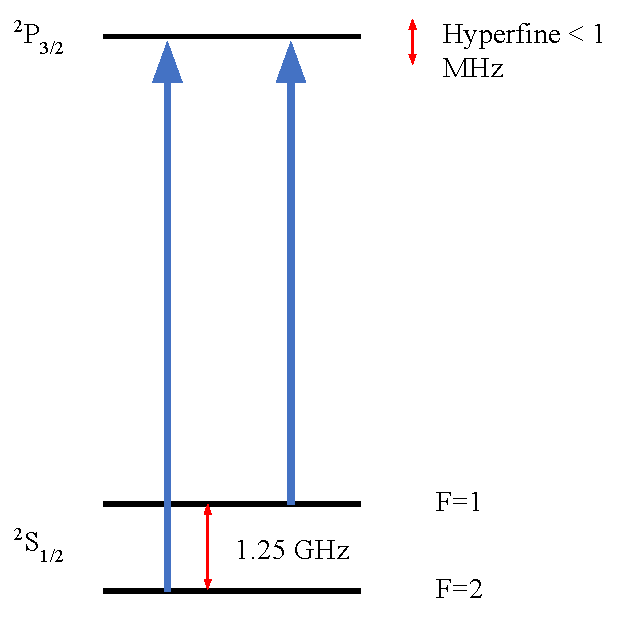
\includegraphics[width=0.6\textwidth]{images/Be_cooling.pdf}
	\caption{Electronic structure of \ce{^9Be+}, laser cooling is done with 313 nm light.}
	\label{fig: Be structure}
\end{figure}

\begin{figure}[H]
	\centering
	\missingfigure{Laser and AOM's}
	\caption{AOM's running at 400 MHz are used to tune the initially blue detuned primary beam on resonance with the \ce{^2S1/2} to \ce{^2P3/2} transition. A double passed AOM tunes the primary beam to the \ce{^2S3/2} to \ce{^2P3/2} transition to re-pump any \ce{^2P3/2 -> ^2S3/2} decays. A third AOM creates a first order beam 200 MHz red to aid the capture of hot ablated \ce{Be+} ions.}
	\label{fig: AOMs}
\end{figure}

As we excite the cooling transition, force is being imparted onto the ion via absorption of the photons and spontaneous emission. We can define the force to be the product of the scattering rate of a two level system and the momentum of each photon.

\begin{align}
	F & = p \Gamma \rho_{pp} \nonumber \\
	& = \hbar k \Gamma \frac{1}{2} \frac{s}{1+s+4\left(\frac{\delta-\vec{k}\cdot \vec{v}}{\Gamma}\right)^2} \label{eq: laser force}
\end{align}

Where $k$ is the photon's wavenumber, $\Gamma$ is the linewidth of the excited transition, and $\rho_{pp}$ is the probability of finding the ion in the excited \ce{^2P3/2} state characterized by the saturation parameter $s = I/I_s=I/(\frac{\pi h c}{3 \lambda^3 \tau})$ and laser detuning $\delta=\omega_0-\omega_l$. We can see that the force the ion feels is dependent on the laser detuning from resonance, which in turn is dependent on the doppler shift of the ion with respect to the laser $\vec{k} \cdot \vec{v}$. In general, the laser frequency ($\omega_l$) is red detuned from the cooling transition ($\omega_l < \omega_0$). In this instance, if the ion is moving towards the laser such that the velocity ($v$) and $k$ vector are anti-aligned, we see a positive doppler shift in the frequency ($+kv$), decreasing the effective detuning, increasing the scattering rate. When the ion is moving away from the laser while $\omega_l < \omega_0$ is true, we see that the detuning increases, lowering the scattering rate. Each time the ion absorbs a photon, it gains a momentum kick in the photon's direction, meaning the ion preferentially absorbs light that causes it to lose momentum. After absorption, the ion emits a photon after $\tau=\Gamma^{-1}$ time, isotropically, which averages to zero. We can Taylor expand equation \ref{eq: laser force} for small values of $v$ to find this velocity dependence.

\begin{equation*}
	F(v) = F(v=0) + \beta v
\end{equation*}

Where we define the damping coefficient:

\begin{equation*}
	\beta= 4 \hbar k^2 \frac{s \frac{\delta}{\Gamma}}{1+s+4\left(\frac{\delta}{\Gamma}\right)^2}
\end{equation*}

Since the ion trap is not a perfect harmonic potential, which would require hyperbolic trap electrodes, the ion's trajectory is mixed along each axis, allowing for the 3 dimensional laser cooling with just one beam angled from both radial and axial axes of the trap.